\documentclass[11pt,oneside]{article}
\usepackage{fullpage}
%%% Load some useful packages:
%% "New" LaTeX2e graphics support.
\usepackage{graphicx}
%%	using final option to force graphics to be included even in draft mode
%\usepackage[final]{graphicx}
%% Tell graphicx the default directory for all figures
\graphicspath{{figures/}}

%% Enable subfigure support
\usepackage{subfigure}

\begin{document}
\title{Dissertation proposal abstract}
\author{Pavel Senin \\
 \texttt{senin@hawaii.edu}
}
\date{July 2009}
\maketitle

\section{Motivation}
Since the first computers were build and first programs written many research was done on understanding of both: programming and programs. In contemporary understanding the human activity called ``\textit{programming}'' consists of many iterative, high-level phases and interleaving activities such as planning, writing, testing, debugging, and maintaining the source code of computer programs. Each of these phases in turn encloses many of low-level continuous processes and episodes. In addition to that, social interactions among developers and between developers and users are adding even more complexity into each phase of the programming \cite{citeulike:5029482}. The computer program (\textit{computer system}, or \textit{software}) itself, from other hands, has it's own lifecycle which is directed by users and a programming effort but also, as observed in many cases, programs, especially large software systems, tend to be ``orchestrating'' all needed programming activities and social interactions \cite{citeulike:5042856}. All of this creates a great process complexity due to unclear dependencies and spurious connections between different activities making an understanding of a software development process and software evolution difficult. The two processes discussed here are highly connected and while differ in context in modern literature they aggregated into the single term: ``\textit{software process}''.

As a systematic study, the ``understanding'' of software process involves measurements, comparisons and validation experiments. Over the years many work has been done in order to discover and standardize metrics for programming activity and a software. Currently we have a rich variety of software utilities aiding the collection and analysis of a software process metrics. All of these findings and available tools created a rich ground for investigation of the software process and many successful work has been done discovering various specific patterns and characterizing metrics and features. Some of this research resulted in a such mature software process models as CMM, ISO, PSP etc. which were recognized as industry standards \cite{citeulike:5043104}.

Nevertheless, software development process stays error-prone and many, more than a half, of all software development projects ending up failing or very poorly executed for many reasons. Some of them getting abandoned running out of budget, some delivered with so low quality or so late that they become useless and some, when delivered, never get used by prospective users because they do not fulfill original requirements. The cost of this lost effort is enormous and it clearly reveals our incomplete knowledge of the software process fueling up continuous research in the field. 

\section{Contribution and Impact}
At the ICS Department of the University of Hawaii we are developing an advance in-process software engineering measurement and analysis system called Hackystat which is aiding our own research in the field of software process. Personally, having three years of experience with Hackystat as a user and participating in the design and development of last two versions of Hackystat for more than two years, I see this software system as an ``one-stop shopping place'' for metrics collection utilities, storage database, analysis engine and visualization modules. The latest Hackystat implementation is a sophisticated distributed, service-oriented system which provides users not only with visualization of all metrics and their derivatives, but aids the understanding of metrics trend dynamics through the system of rules and alarm indicators. What the system is lacking in my opinion is it's own intelligent ability to discover novel rules and patterns in the software process and connecting them with some known phenomena. Currently I am conducting research, developing software tools and planning validation experiments in effort to cover this gap.

I am developing a Hackystat module called Trajectory which will aid the discovery of a novel knowledge about the software process through the utilization of unsupervised learning algorithms altered to the domain specificity. This module will alleviate the existing complexity of the in-process and post-process analyses, that are performed mostly manually, through the ``eyeballing'', and require an advance (expert level) understanding of both: process metrics and the underlying generative processes. By utilizing current state of the art knowledge discovery and data mining algorithms and a domain knowledge, Trajectory software will provide user with discovered strong episodal and sequential patterns as well as with ``surprise'' patterns, which frequency is highly different from the expected one. Implementation of the clustering algorithms will also aid the classification analyses of the Hackystat telemetry streams.

\section{Approach and Methods}
The Hackystat system, while stores all of the richness of data collected from sensors, has several layers of abstraction before presenting this data to the user. By employing these features, my system is fed by a set of daily aggregated telemetry streams which represent full spectrum of process and software metrics. After these data streams getting normalized, they are indexed with Symbolic Aggregate approXimation algorithm \cite{citeulike:2821475} and once built, indexes stored in the dedicated relational database. The indexing performed by using a sliding window and index encapsulates a full set of found subsequences (temporal motifs) with their frequencies and positions. 

By using a relational database for storage it is possible to address most of KDD and clustering algorithms data requirements with SQL queries, for example in current implementation it's very easy to get the motif frequency vectors for each of the streams, find most frequent temporal motifs across the subset of streams etc. This rich data field allows to perform further analyses with time-points and time-intervals data models as well. For time-points data I am planning to experiment with Interagon Query Language (IQL) for symbolic temporal data \cite{citeulike:5043086}, AprioriAll \cite{citeulike:775528} and Pattern-Growth algorithms \cite{citeulike:5043097} as well as with Episodes \cite{citeulike:5043099} and Partial Order patterns \cite{citeulike:5043101}. For time-interval data I will investigate applicability of Allen's interval algebra \cite{citeulike:191348} and it's derivatives (UTG \cite{citeulike:5043086} and TSKR\cite{citeulike:3978076}) for the software process domain. 

While all of these are generic methods and algorithms for temporal data mining, and as pointed in many work, tend to generate overwhelming amount of spurious data I am planning to constraint the search space and prune resulting patterns by applying a domain-specific knowledge.

\section{Current state of the research}
Description of the current software implementation, planned process of KDD and demonstration of the preliminary results - 1 page.

\begin{figure}[tbp]
   \centering
   \includegraphics[height=65mm]{system_overview.eps}
   \caption{The high-level system overview. Data collected from users and integration system collected and aggregated by Hackystat, later SAX indexes built. Data mining tools perform unsupervised pattern discovery on demand constrained by the domain knowledge. The GUI provides interface for discovered patterns and knowledge base aiding iterative refinement of knowledge.}
   \label{fig:system_overview}
\end{figure}


%%% Input file for bibliography
\bibliography{seninp}
%% Use this for an alphabetically organized bibliography
\bibliographystyle{plain}

\end{document}
